\documentclass[11pt]{beamer}
\usetheme{CambridgeUS}
%\usetheme{Boadilla}
%\usecolortheme{beaver}
\usepackage[utf8]{inputenc}
\usepackage[francais]{babel}
\usepackage[T1]{fontenc}
\usepackage{amsmath}
\usepackage{amsfonts}
\usepackage{amssymb}
\usepackage{graphicx}
\usepackage{eurosym}
\usepackage[percent]{overpic}
\usepackage{hyperref}
\usepackage[final]{pdfpages}

\author{N. BALLET — B. CORTIER – L. LAZARE}
\institute[]{UTBM}
\title{Génération d'objets paramétriques}
\subtitle{Projet d'IN55}
%\setbeamercovered{transparent}
%\setbeamertemplate{navigation symbols}{}
%\logo{\includegraphics[width=0.12\textwidth]{utbm}}
%\institute{}

\date{\today{}}

\subject{Génération d'objets paramétriques}

\graphicspath{{fig/}}

\beamertemplatenavigationsymbolsempty{} % remove navigation symbols.

%\setbeamertemplate{blocks}[rounded][shadow=false]

\begin{document}

\begin{frame}
    \titlepage{}
\end{frame}

\begin{frame}{Sommaire}
    \tableofcontents
\end{frame}

\section{Génération d'objet paramétrique~: le diamant}

\begin{frame}{Génération des points}
    {\centering 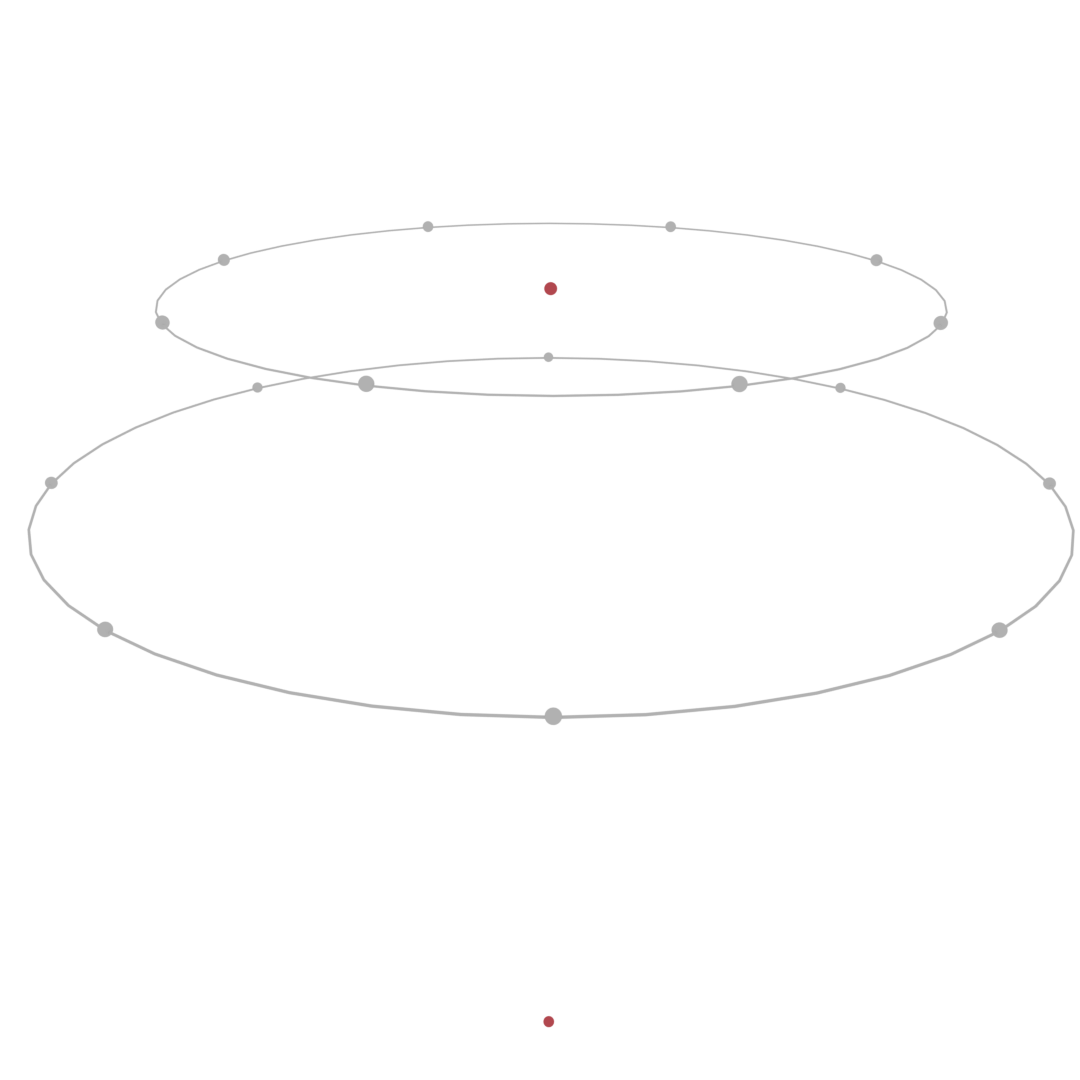
\includegraphics[height=0.95\textheight]{Maillage/circles}}
\end{frame}

\begin{frame}{Génération des faces}
    {\centering 
\includegraphics[height=0.95\textheight]{Maillage/wireframe}}
\end{frame}

\begin{frame}{Résultat}
    {\centering 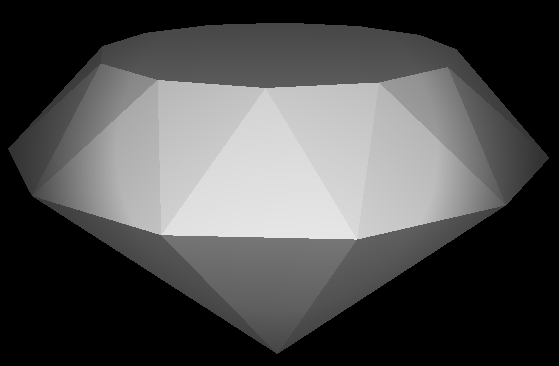
\includegraphics[height=0.95\textheight]{Maillage/result}}
\end{frame}

\section{Éclairage à l'aide de la méthode de Phong}

\begin{frame}
    Gestion des trois composantes de Phong~:
    \begin{itemize}
        \item composante ambiante
        \item composante diffuse (gestion de la diffusion de la lumière au sein d'une face)
        \item composante spéculaire (gestion des reflets).
    \end{itemize}

    Différents types de lumières~:
    \begin{itemize}
        \item lumière directionnelle
        \item lumière localisée
        \item projecteur.
    \end{itemize}

    Notre implémentation nous permet de gérer un nombre arbitraire de lampes, le chiffre exact étant défini par des constantes
    se trouvant dans le \textit{fragment shader} (configuré de manière arbitraire sur 5 lumières directionnelles, 15 lumières localisées et 15 spots au maximum).
\end{frame}

\begin{frame}
    {\centering 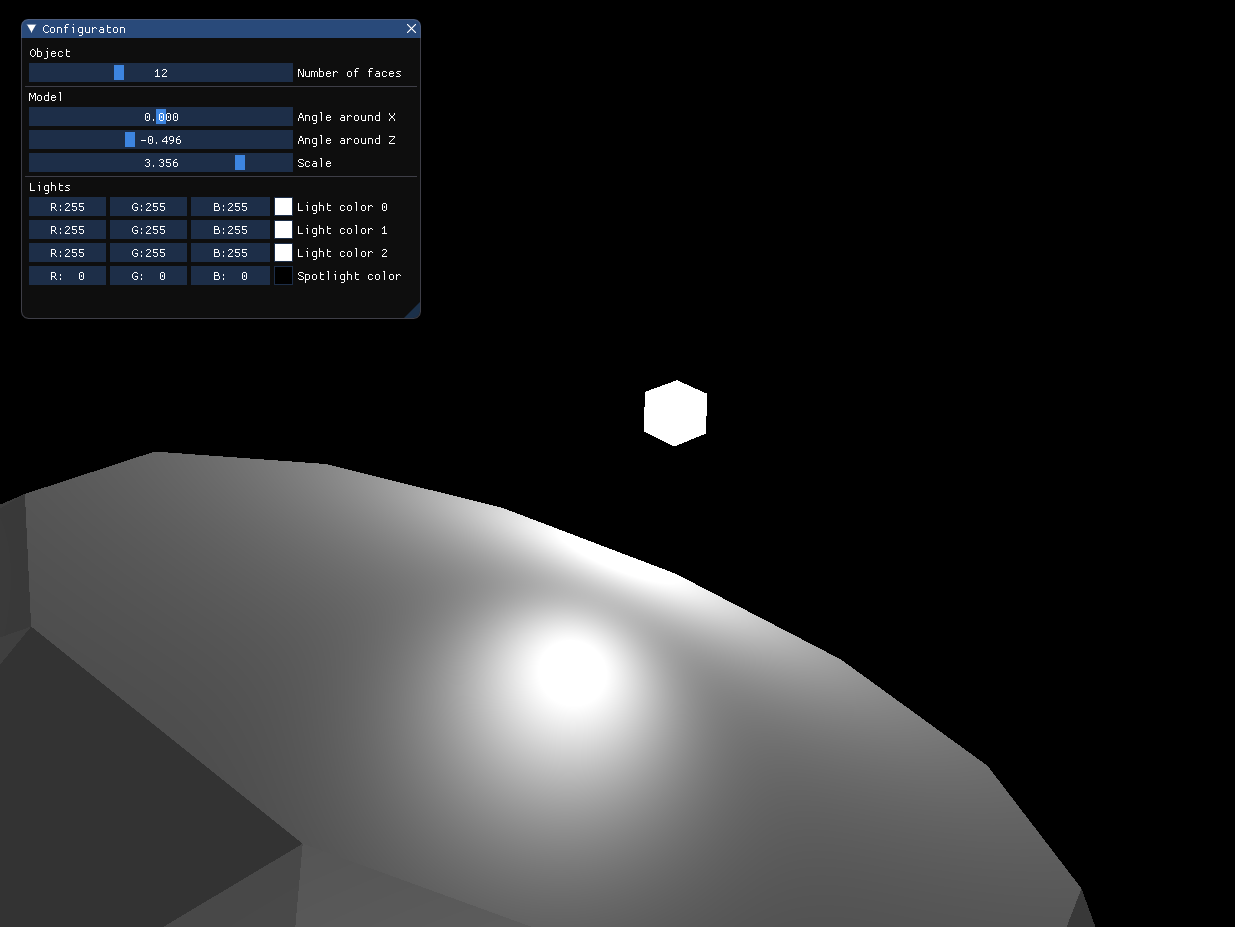
\includegraphics[width=0.9\textwidth]{screenshot_software_3}}
\end{frame}

\section{Réflexions sur le diamant}

\begin{frame}
    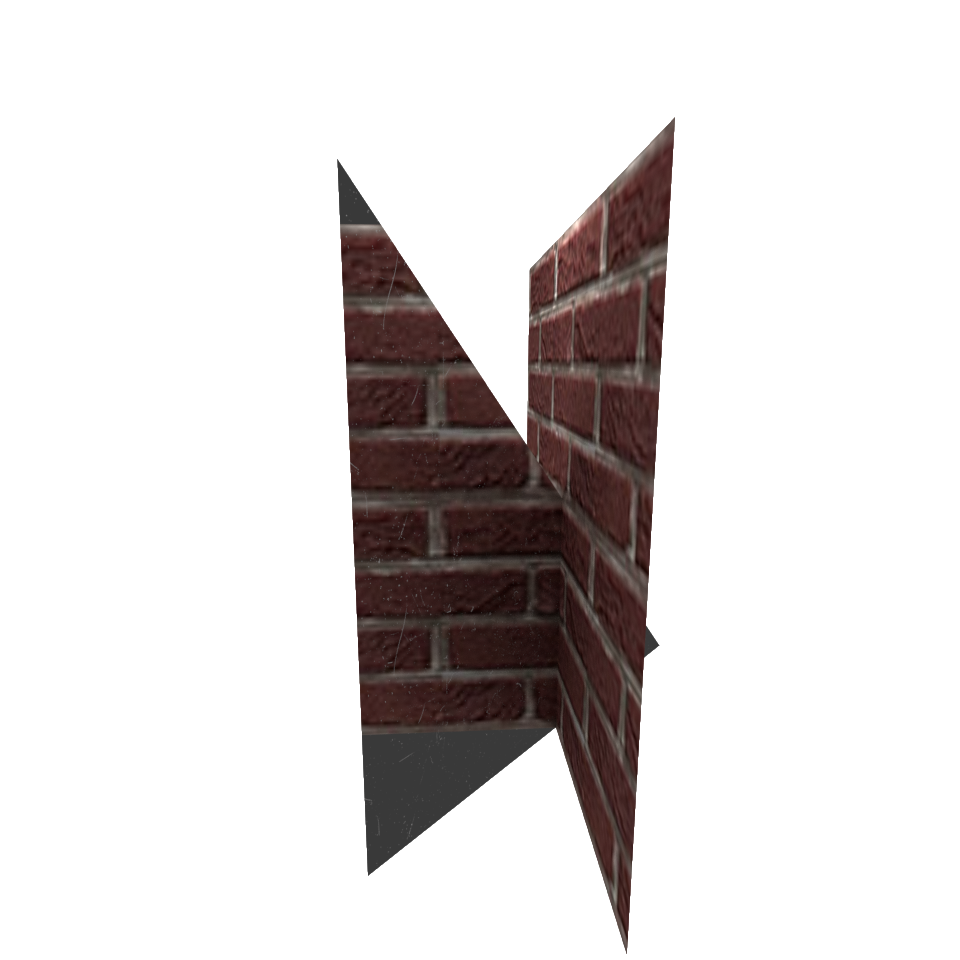
\includegraphics[width=0.45\textwidth]{Reflexion/1}
    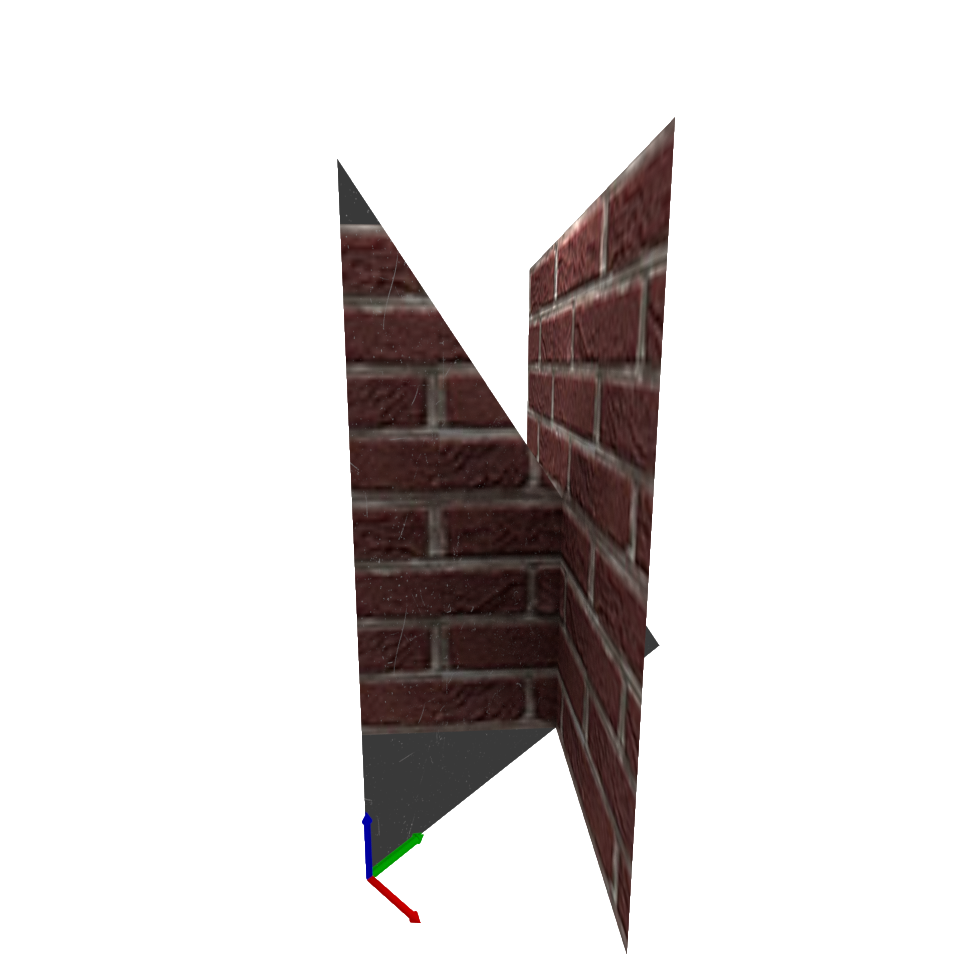
\includegraphics[width=0.45\textwidth]{Reflexion/2}
\end{frame}

\begin{frame}
    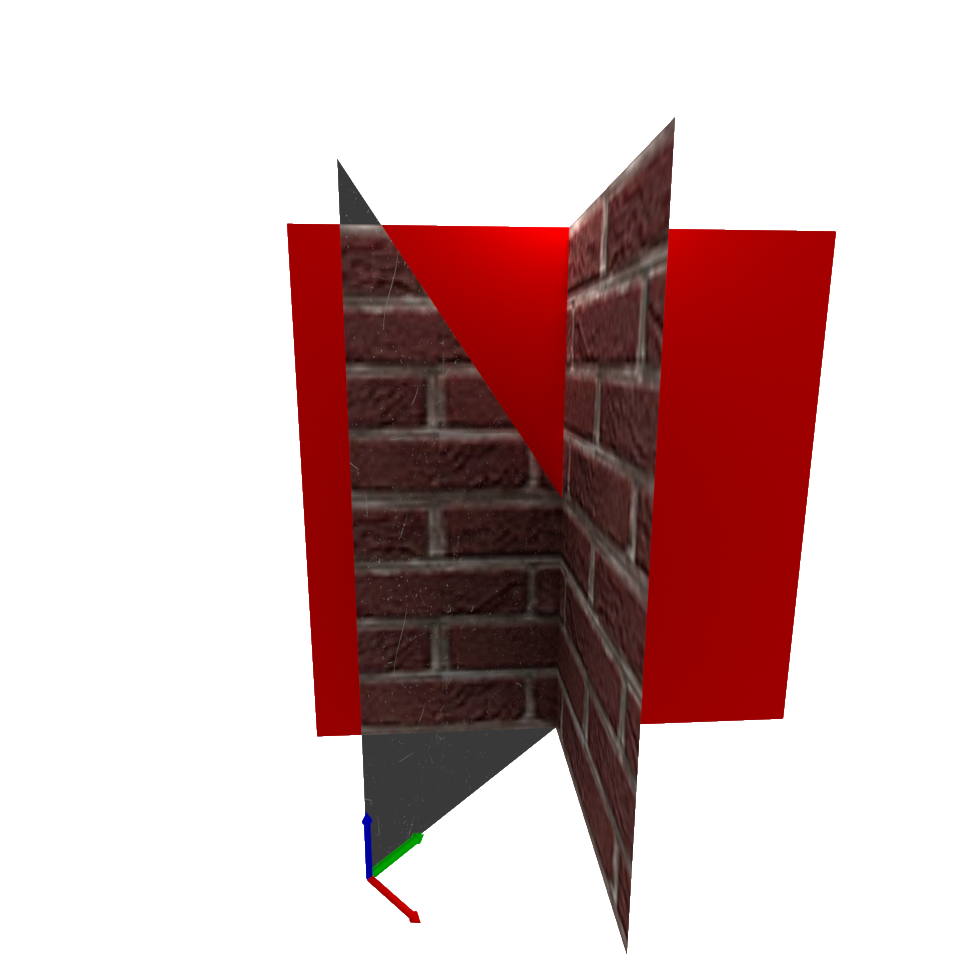
\includegraphics[width=0.45\textwidth]{Reflexion/3}
    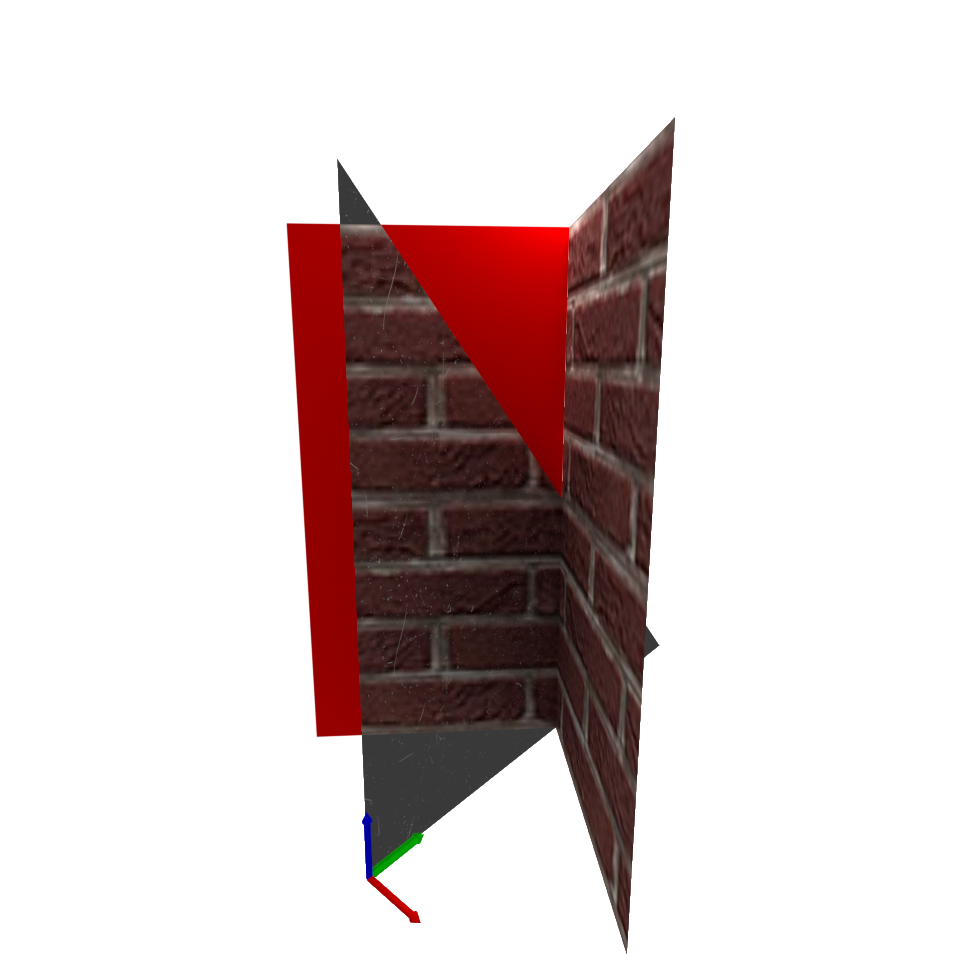
\includegraphics[width=0.45\textwidth]{Reflexion/4}
\end{frame}

\begin{frame}
    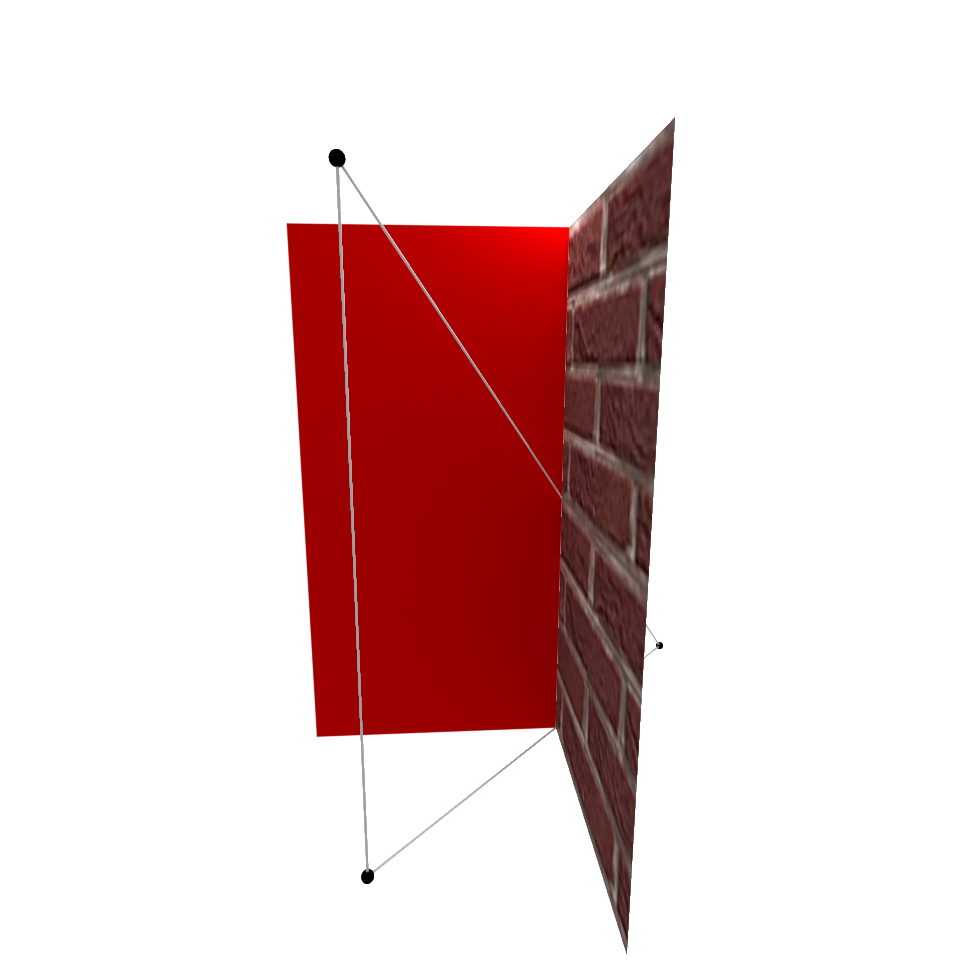
\includegraphics[width=0.45\textwidth]{Reflexion/5}
    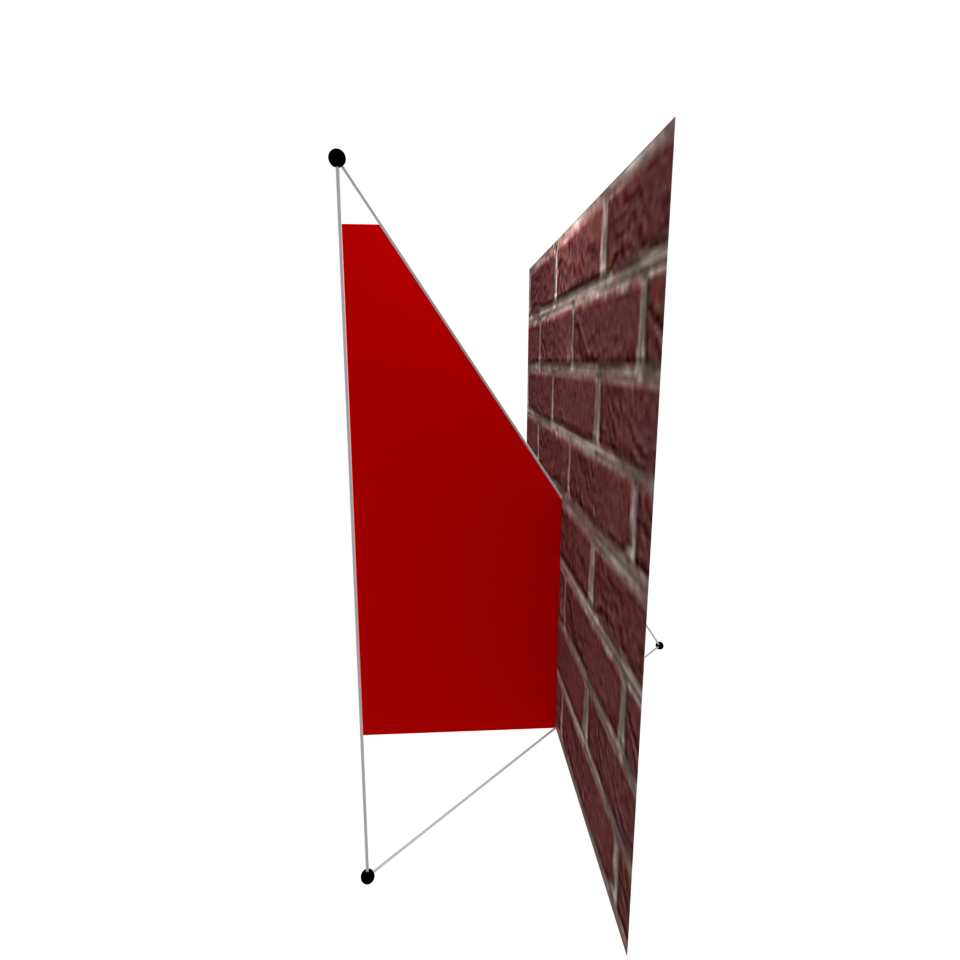
\includegraphics[width=0.45\textwidth]{Reflexion/6}
\end{frame}

\end{document}

